\section{Overview}
By developing the unified representation for both data and domain knowledge, and utilizing ontological annotations, we can produce one RDF hypergraph, which serves as the basis for semantic data mining. Given this, the main research challenge is how to utilize the data and ontology together for semantic data mining. In this dissertation, we focus on one important data mining tasks, the {\em frequent pattern mining}, to showcase the utility of RDF hypergraphs.

\subsection{Frequent Pattern Mining}
\label{sec:association}
Frequent itemsets play an essential role in many data mining tasks that try to discover interesting relations between features in large databases. In the traditional sense, an itemset is called frequent if its support (number of times the itemset occur in the dataset) is no less than a given threshold. The original motivation for searching association rules came from the need to analyze supermarket customer behavior in terms of products that are often purchased together. However, it is evident that the measure of support essentially restrains pattern discovery to account for only directly associated items (\eg, products purchased together) while ignoring possible indirect associations. A prominent example of such indirect association was given by Swanson's land mark paper published in 1987~\cite{swanson87} that described the relationship between fish oil and Raynauld's syndrom through their mutual connections with certain changes in blood.

Such indirect associations can be best captured by graphs. In general, an object set endowed with pairwise relationships can be conceptually viewed as a graph in which vertices represent objects, and any two vertices that have some kind of relationship are joined together by an edge. In this sense the traditional measure of support evaluates the significance of a itemset by the number of direct edges (1-hop path) between item nodes. Extending this notion to allow paths with arbitrary lengths to be taken into account, we are able to evaluate the significance of an itemset in terms of the indirect connections among its nodes. From here on, we call the itemset associated by the indirect connection via multi-hop paths the \emph{semantically associated itemset}, or simply the \emph{semantic association}. In this chapter, We focus on describing graph-based algorithms to find semantically associated itemsets.

The term \emph{semantic association} conforms with the definition proposed by Sheth et al.~\cite{ShethEtal05JDBM} for semantic association between entities in an RDF graph. Specifically, they define the semantic association based on if there exists a sequence of interconnected links between two given entities. In our study of semantically associated itemsets in transaction data, the link between entities can be as simple as the `co-occurrence' relationship if more complicated relationships in ontologies are not concerned. Under Sheth et al's definition, the semantic association between transaction items $i_0$ and $i_n$ can be established by identifying a link of the form $i_0, P_c, i_1, P_c, \ldots , i_{n-1}, P_c, i_n$, in which $P_c$ denotes the property that connects two items (\eg, co-occurrence). Given this, the problem of finding meaningful semantic association becomes how to define a proper graph representation and effective analysis methods that can be carried out to evaluate the strength of semantic associations.

We first rule out simple graphs as the candidate model for discovering semantic associations due to the ambiguity and information loss. For illustrating this point of view, let us consider a relational table depicted in Figure~\ref{fig:hg_and_rg}(a). One can construct a simple undirected graph where the set of vertices is the set of relational attributes (column items) and an edge joins two vertices if the they co-occur in a tuple (as illustrated in Figure~\ref{fig:hg_and_rg}(b)). This graph is called \emph{Gaifman graph}~\cite{Hodkinson02finiteconformal} of a relational structure. The undirected graph can be further enriched by assigning to each edge a weight equal to the support of the 2-itemset consisting of vertices incident to the edge. Cliques (complete subgraphs) in the Gaifman graph, or \emph{Gaifman cliques} for short, are of particular interest because every tuple (ground atom) in data corresponds to a Gaifman clique. However, ambiguity arises as not all Gaifman cliques have matching tuple in the data. There exists cases where cliques are incidental in the sense that several relational ground atoms play together to induce a clique configuration in the Gaifman graph, but no ground atom covers the entire clique (e.g., the clique of $\{A,B,C,D\}$ in Figure~\ref{fig:hg_and_rg}(b) does not correspond to any tuple in the relational table). Further more, given the Gaifman graph we lose the information of how nodes are related. For example, if $A, B$ and $C$ are products purchased by a particular customer as indicated by a record in the transactional table, this information is no longer available in the graph

The RDF bipartite graph introduced in~\ref{sec:graph-rep-for-rdb} comes to remedy as it maximally preserves the semantics in the original table and contains no ambiguity. Plus it is able to represent ontologies in the same way so that analysis approaches on the RDF bipartite graph can systematically utilize information from both data and domain knowledge. Moreover, if a mining task does not involve the use of domain knowledge from ontologies, the RDF bipartite graph can be transformed to a more compact form that achieves better scalability. In the rest of this chapter, we describe in detail the methods for discovering semantically associated itemsets with and without the incorporation of ontologies respectively.

\subsection{Graph-based similarity}
Data mining algorithms rely on the notion of similarity between data points to make meaningful inferences. When data is in $\mathbb{R}^d$, the standard similarity measure is the Euclidean distance. When data has an explicit link structure, shortest path distance is commonly used. However, neither of these measures incorporates the intuition that two data points are similar to each other if they are connected by a high density region. This latter concept of similarity measure has been shown in experiments to lead to significant improvement in a number of learning tasks, see, for example, (Blum \& Chawla, 2001; Corduneanu \& Jaakkola, 2003; Bous-quet et al., 2004)~\cite{}.

Take the simple graph in Fig.~\ref{fig:graphcomp}(B) for example, suppose given a task of friend recommendation based on the information in this graph, the interesting question is whether $c$ or $e$ is a better choice of recommendation to $a$. To answer this question, it is natural to compare the similarity measures $s(a, c)$ and $s(a, e)$. In a rough sense, on can identify in the hypergraph representation that there are two paths between $a$ and $c$ (the formal definition for paths in hypergraphs will be given in Section~\ref{sec:rw_hyper}), while only one between $a$ and $e$. It's intuitive to conclude that $a$ and $c$ are more similar, or closer, than $a$ and $e$. This gives us a hint that meaningful similarity measures on the graph should satisfy the following intuitions:
\begin{enumerate}
\item The more paths connecting two nodes, the closer they are.
\item The shorter the paths, the closer they are.
\end{enumerate}
In other words, the more ``short" connections between two given nodes, the more similar those nodes are. 
To this end, we propose to employ the following quantities as the candidate similarity measure since both of them have the desired property. They are, namely, the \emph{commute time distance} based similarity measure from the random walk model on hypergraph, and the inner product similarity based on the \emph{pseudoinverse of the hypergraph Laplacian}. 
Several measures derived from random walk on graphs have been shown to possess such desired property. In the following example, we quantitatively show the property of commute time distance, which characterizes the expected number of steps to take a round trip between a starting node and a target node.

\begin{figure}[tbh]
\centering
\begin{minipage}[c]{\textwidth}\centering
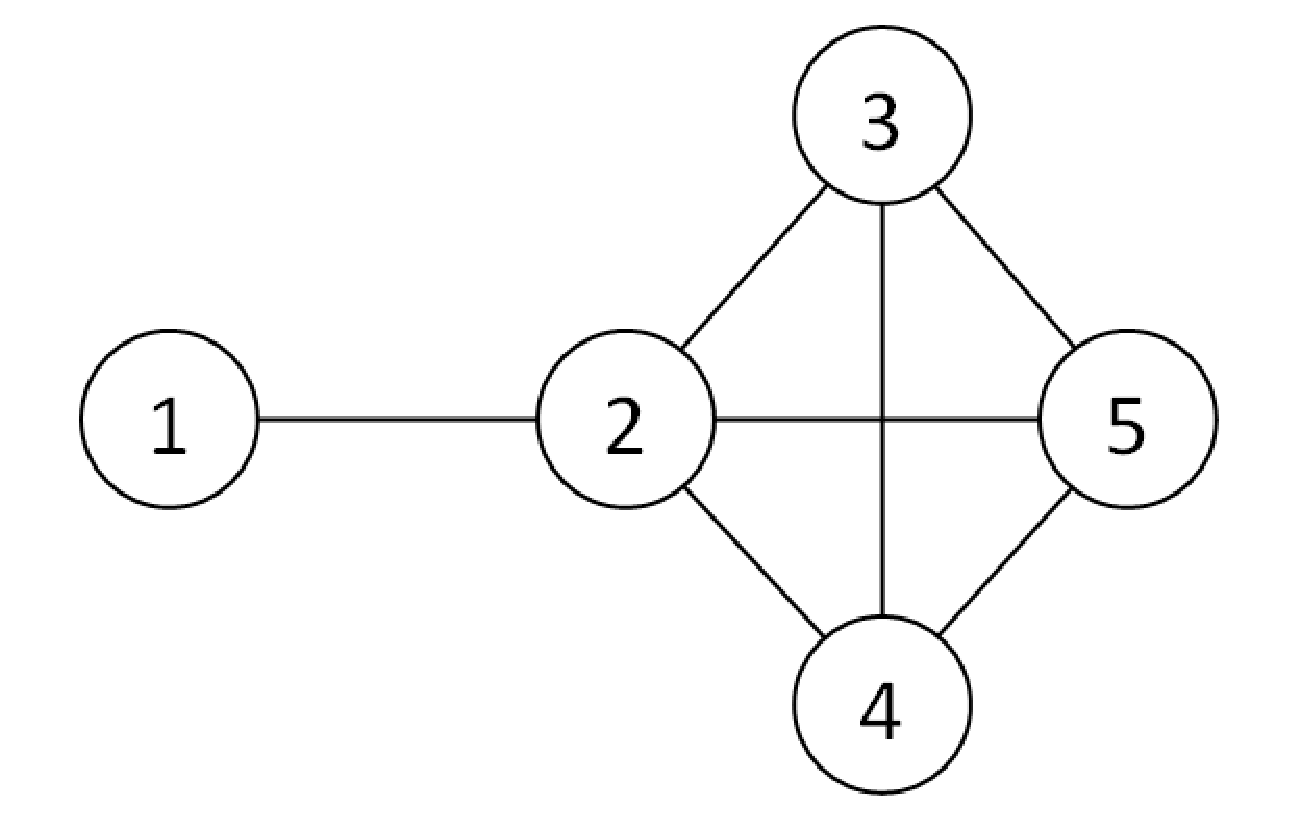
\includegraphics[width=.4\textwidth]{fig/comm-dist-demo.eps}
\end{minipage}
\hfill
\begin{minipage}[c]{\textwidth}\centering
\begin{tabular}{r|r|r|r|r|r || r|r|r|r|r}
\hline\hline
\multicolumn{6}{c||}{Euclidian Distance}	&	\multicolumn{5}{c}{Commute Distance}		\\
\hline\hline							
Index	&	1	&	2	&	3	&	4	&	5	&	1	&	2	&	3	&	4	&	5	\\
\hline
1	&	0	&	1	&	1.85	&	1.85	&	2.41	&	0	&	12.83	&	19.79	&	19.79	&	20.34	\\
\hline
2	&	1	&	0	&	1	&	1	&	1.41	&	12.83	&	0	&	6.96	&	6.96	&	7.51	\\
\hline
3	&	1.85	&	1	&	0	&	1.41	&	1	&	19.79	&	6.96	&	0	&	7.51	&	6.96	\\
\hline
4	&	1.85	&	1	&	1.41	&	0	&	1	&	19.79	&	6.96	&	7.51	&	0	&	6.96	\\
\hline
5	&	2.41	&	1.41	&	1	&	1	&	0	&	20.34	&	7.51	&	6.96	&	6.96	&	0	\\
\hline\hline
\end{tabular}
\end{minipage}
\caption{\label{fig:cd-demo}}
\end{figure}

Figure~\ref{fig:cd-demo} shows a graph of five nodes with a specific edge configuration (the so called ``lollipop graph''). The Euclidean distance between each pair of nodes are shown in the left-hand side of the corresponding table above and the respective commute time distance are shown on the righ-hand side. It can be seen that node 1 and node 3 are equally close to node 2 in terms of their Euclidean distances. However, node 2 and 3 are considered much closer under commute time distance because they are within a much more densely connected subgraph. This shows that, unlike Euclidean distance and shortest path distance, commute distance between two nodes captures both the length of paths between them and their local neighborhood densities. We believe such property makes the commute time distance a suitable measure for graph-based data mining algorithms. We also explore other random walk-based measures including the pseudoinverse of the Laplacian matrix and the stationary probability that are closely related to commute time distance. In the following, we first describe random walk on simple graph and then introduce the extension to hypergraph. The details of hypergraph-based similarity measures are described in the subsequent sections. 
%These methods are described in detail in the following sections and trade-offs between them are studied.

\subsubsection{Random Walk}
\textbf{Random Walk on Simple Graph}
Given a graph and a starting point we select a neighbor of it at random and move to this neighbor then we select a neighbor of this point at random and move to it etc. The random sequence of points selected this way is a random walk on the graph. In other words, a random walker can jump from vertex to vertex and each vertex therefore represents a state of the Markov chain. The average first-passage time $m(k|i)$~\cite{randomwalks} is the average number of steps needed by a random walker for reaching state $k$ for the first time, when starting from state $i$. The symmetrized quantity $n(i,j)=m(j|i)+m(i|j)$ called the average commute time~\cite{randomwalks}, provides a distance measure between any pair of states. The fact that this quantity is indeed a distance on a graph was proved independently by Klein and Randic~\cite{Klein} and Gobel and Jagers~\cite{Gobel}.

The Laplacian matrix $\mathbf{L}$ of a graph is widely used for finding many properties of the graphs in spectral graph theory. Given node degree matrix $\mathbf{D}$ and graph adjacency matrix $\mathbf{A}$, the Laplacian matrix of the graph is defined as $\mathbf{L}=\mathbf{D}-\mathbf{A}$. The normalized Laplacian is given by $\mathbf{L}_N=\mathbf{I}-\mathbf{D}^{-1/2}\mathbf{A}\mathbf{D}^{-1/2}$, where $\mathbf{I}$ is the identity matrix. The average commute time $n(i,j)$ can be computed in closed form from the Moore-Penrose pseudoinverse of $\mathbf{L}$~\cite{pseudo}, denoted by $\mathbf{L}^+$.

Various quantities derived from random walk on graph has been used in a number of applications. Fouss et al.~\cite{Fouss06random-walkcomputation} compared twelve scoring algorithms based on graph representation of the database to perform collaborative movie recommendation. Pan et al.~\cite{Pan} developed a similarity measure based on random walk steady state probability to discover correlation between multimedia objects containing data of various modalities. Yen et al.~\cite{Yen05clusteringusing} introduced a new k-means clustering algorithm utilizing the random walk average commute time distance. Zhou et al.~\cite{Zhou:2009:GCB:1687627.1687709} presented a unified framework based on neighborhood random walk to integrate structural and attribute similarities for graph clustering.

\textbf{Random Walk on Hypergraph}
\label{sec:rw_hyper}
We can associate each hypergraph with a natural random walk which has the transition rule as described in~\cite{Zhou06learningwith}. Given the current position $u \in V$; first choose a hyperedge $e$ over all hyperedges incident with $u$ with the probability proportional to $w(e)$; and then choose a vertex $v \in e$ uniformly at random. Obviously, it generalizes the natural random walk defined on simple graphs. Let $\mathbf{P}$ denote the transition probability matrix of this hypergraph random walk.
Then each entry of $\mathbf{P}$ is
\[
p(u,v) = \sum_{e\in E}{w(e)\frac{h(u,e)}{d(u)}\frac{h(v,e)}{\delta(e)}}\, .
\]
In matrix notation, $\mathbf{P}=\mathbf{D}_v^{-1}\mathbf{HWD}_e^{-1}\mathbf{H}^T$.
Zhou et al.~\cite{Zhou06learningwith} define the following normalized hypergraph Laplacian $\mathcal{L}$ based on the random walk model:
\begin{align}
\mathcal{L}=\mathbf{I}-\mathbf{\Theta},   ~\mathrm{where}~ \mathbf{\Theta}=\mathbf{D}_v^{-\frac12}\mathbf{HWD}_e^{-1}\mathbf{H}^T\mathbf{D}_v^{-\frac12} \label{eq:normalizedHyperL}.
\end{align}

\section{Mining Semantically Associated Itemsets without Ontologies}
In this section, we present our study for discovering semantically associated itemsets based on hypergraph without incorporating domain knowledge in ontologies. The goal of this study is to show that, using graph based formalism, we can obtain interesting patterns that are unable to be captured by traditional methods. 

If a mining task does not involve the usage of ontologies and focuses only on data in tables, we can use an alternative hypergraph representation that is more compact than the RDF bipartite graph to model the data. The process to generate such hypergraph is called \emph{RDF hypergraph coarsening} as described in Definition~\ref{def:hg-coarsen}.

\subsection{RDF Hypergraph Coarsening}

\begin{figure}[tbh]
\centering
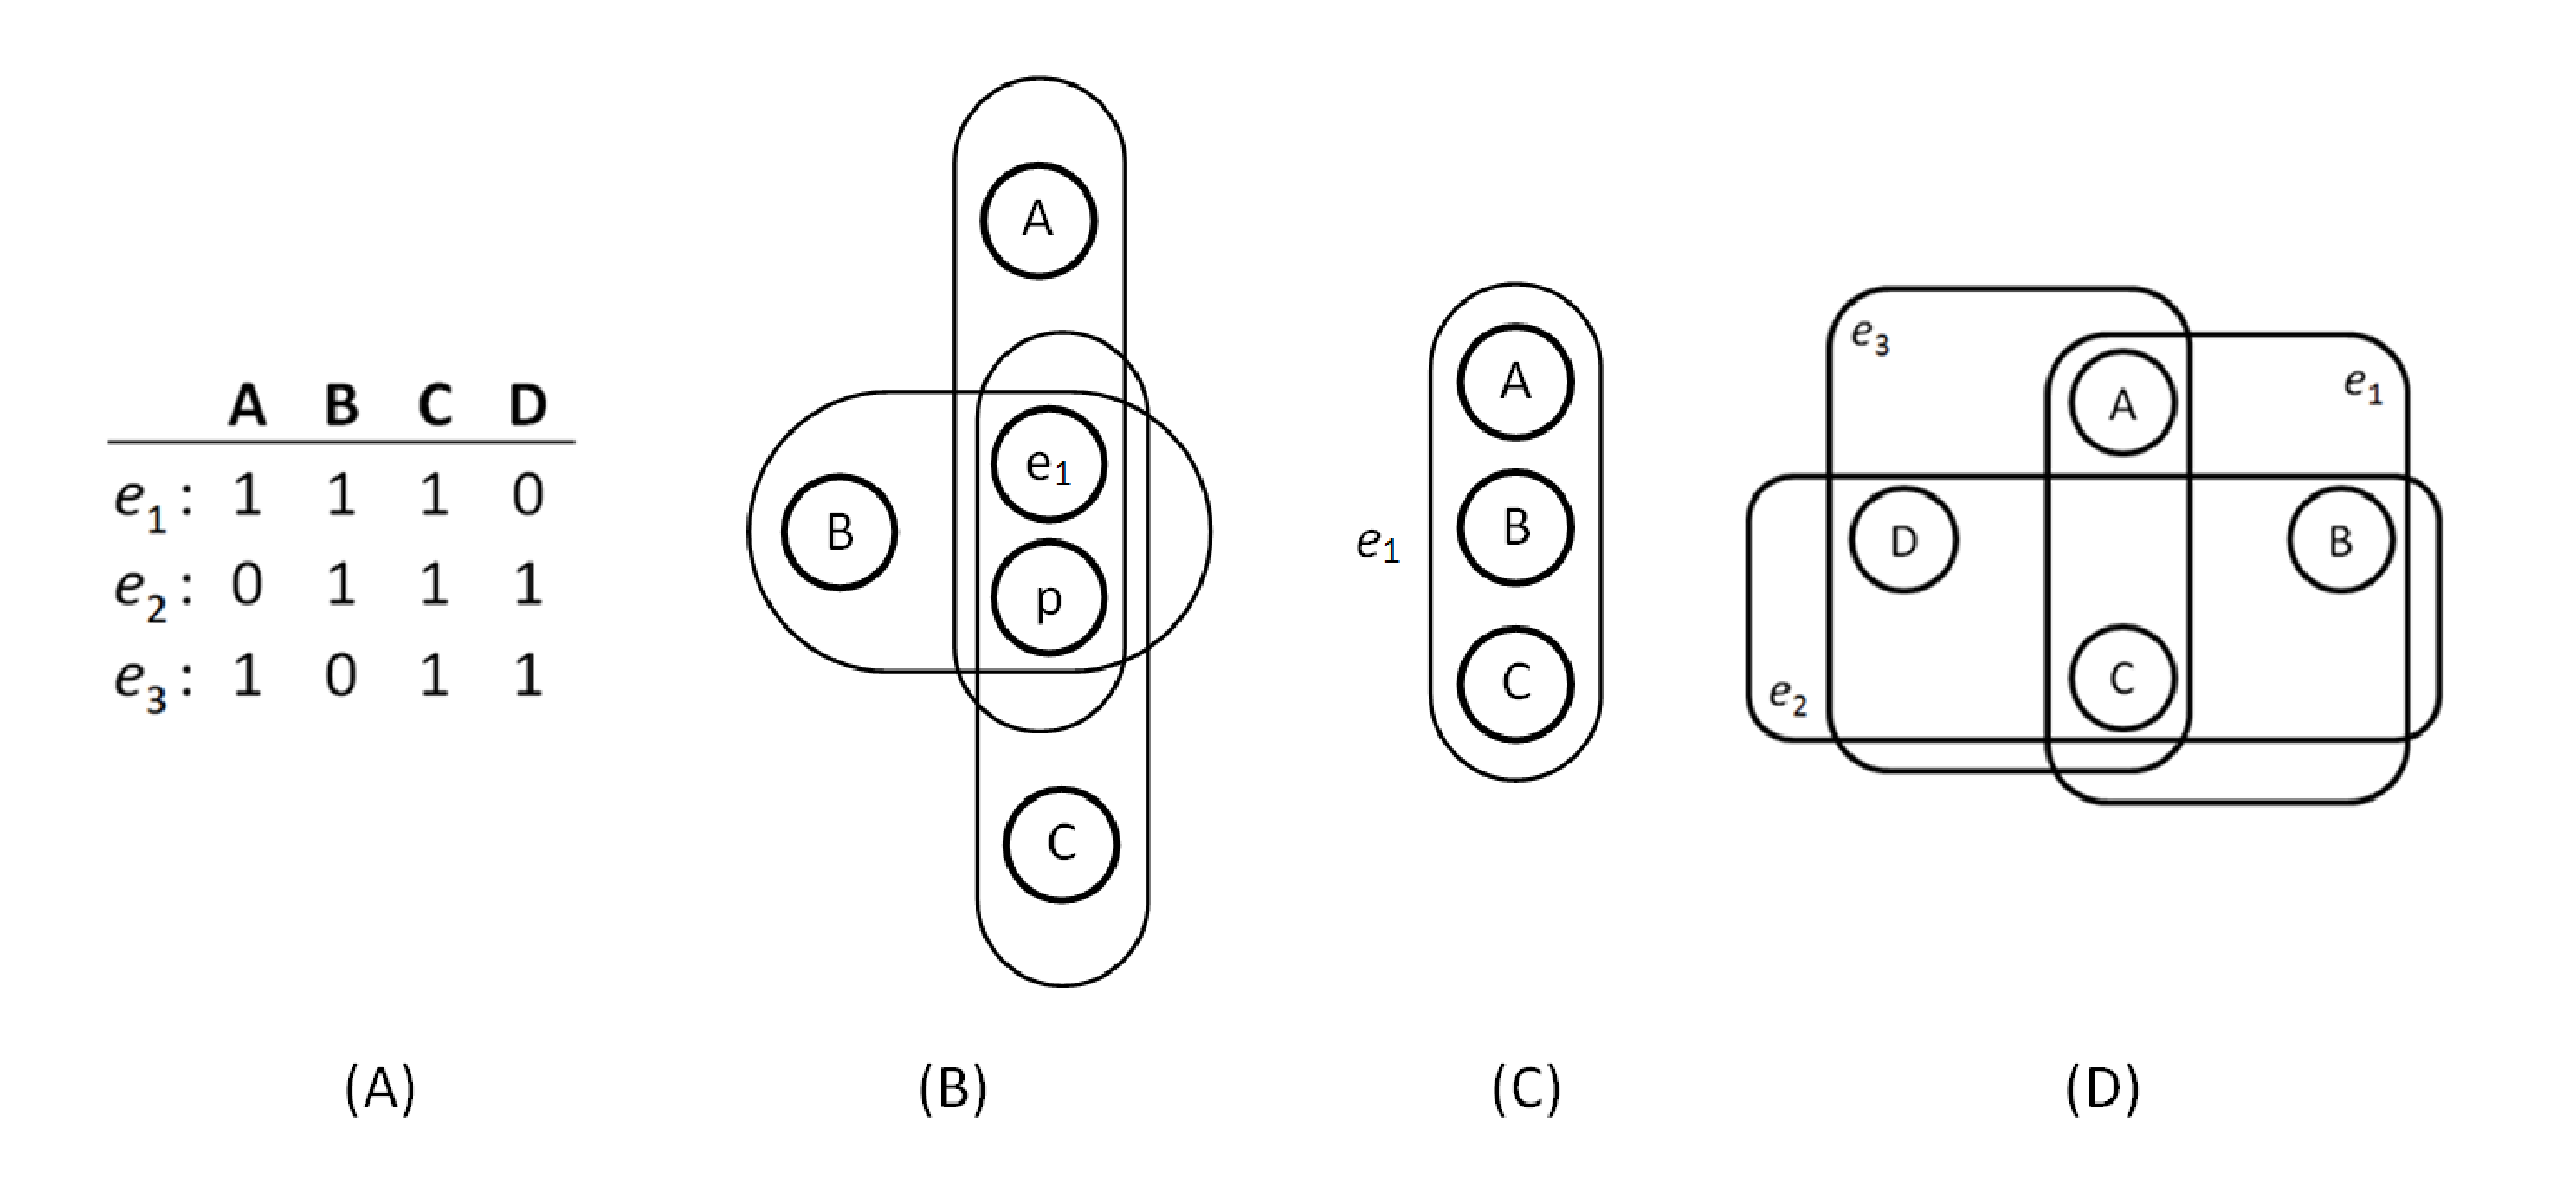
\includegraphics[width=\textwidth]{fig/hypergraph-coarsening.eps}
\caption{\label{fig:hypergraph-coarsening} .}
\end{figure}

\begin{mydef}[\textbf{RDF hypergraph coarsening}]
\label{def:hg-coarsen}
RDF hypergraph coarsening is the process of computing a compact form given an input RDF hypergraph for a relational table by merging vertices into larger groups and removing less significant vertices. The choice of vertices is pertinent to the specific mining tasks. Note that RDF hypergraph is 3-uniform and in the case of RDF hypergraph for relation tables, each hyperedge has three nodes corresponding to the RDF statement of the form \texttt{<row>, <p>, <column>}. The \texttt{<p>} node is the auxiliary predicate denoting the context-dependent semantic relationship between the row and column nodes (\eg, such as that can be as general as \texttt{<mentions>}), and since it is incident to all RDF hyperedges it is first removed in the coarsening process as it bears the least amount of information. Next, if the mining task focuses on discovering patterns among column nodes (\eg, frequent pattern mining), we can merge column nodes that coincide with the same row nodes into a new hyperedge and subsequently remove the row node, and vice versa for mining tasks focusing on row nodes.
\end{mydef}

\begin{myexp}[\textbf{Generation of a column-wise hypergraph for a relational table}]
\label{column-wise-hg}
Figure~\ref{fig:hypergraph-coarsening} (A) shows a sample relational table. Using the method described in Example~\ref{exp:repBinRDB} we can represent this binary-valued table to an RDF hypergraph as is shown in Figure~\ref{fig:hypergraph-coarsening} (B), which demonstrates three hyperedges corresponding to the first row in the table created by transforming the row into three RDF statements, i.e., \texttt{<$e_1$, p, A>, <$e_1$, p, B>}, and \texttt{<$e_1$, p, C>}. Figure~\ref{fig:hypergraph-coarsening} (C) illustrates the coarsened hypergraph according to Definition~\ref{def:hg-coarsen}. Supposing we are interested in discovering relationship between column nodes \texttt{A, B} and \texttt{C} in a frequent pattern mining task, we can remove the nodes \texttt{$e_1$} and \texttt{p} that are commonly incident to all the three hyperedges, and then merge nodes \texttt{A, B} and \texttt{C} to form a single hyperedge. Figure~\ref{fig:hypergraph-coarsening} (D) shows the resulting coarsened hypergraph for the relational table in Figure~\ref{fig:hypergraph-coarsening} (A).
\end{myexp}

Given the method for RDF hypergraph coarsening, we propose to construct a coarsed hypergraph for the relational table in the scenario where ontologies are not included. The relational attributes constitute the universe of vertices in the hypergraph. Based on this hypergraph, our approach for mining semantically associated itemsets starts by first generating 2-itemsets. A 2-itemset $\langle i,j \rangle$ is considered semantically associated if the hypergraph-based similarity measure $s(i,j)$ exceeds some threshold. In the following, we describe two similarity measures $s_{CT}$ and $s_{L+}$ based on, respectively, the average commute time distance on hypergraph and the inner-product-based representation of the pseudoinverse of Hypergraph Laplacian. Given discovered semantically associated 2-itemsets, we propose a hypergraph expansion method along with two search strategies, namely, the clique and connected component search, in the resulting graph for finding semantically associated $k$-itemsets ($k>2$).
\begin{figure*}[tbh]
\begin{center}
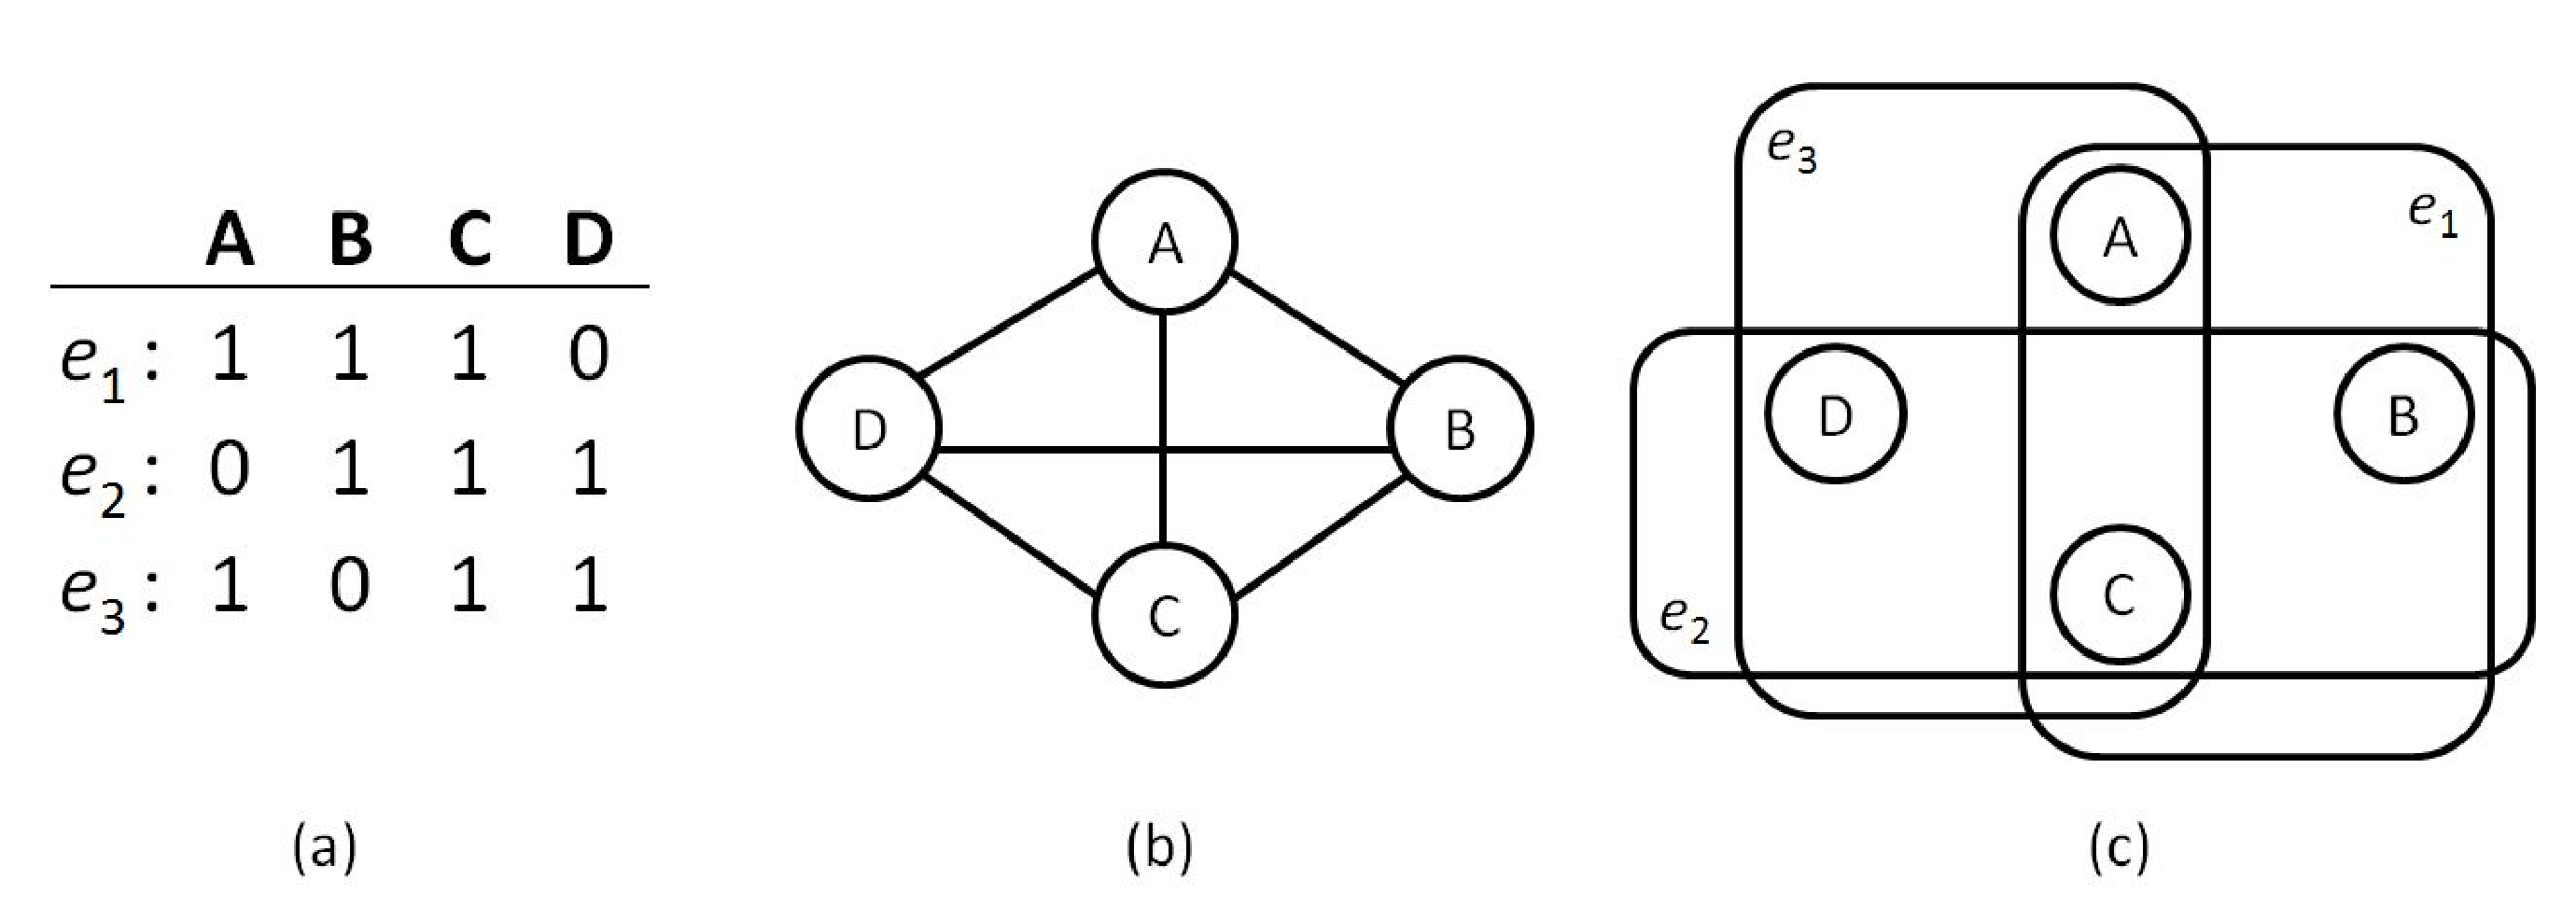
\includegraphics[width=.8\textwidth]{fig/hg_and_rg1.eps}
\end{center}
\caption{\label{fig:hg_and_rg} (a) an example transaction table; (b) the Gaifman graph representation of the table; (c) The hypergraph representation of the table}
\end{figure*}

\subsubsection{Methods for Generating 2-itemsets}
In the following we describe two similarity measures that define the strength of bond between a pair of semantically associated items.

\textbf{Average Commute Time Similarity $s_{CT}$}\\
To compute commute-time distance between vertices in a hypergraph, we need to first define the combinatory hypergraph Laplacian $\mathbf{L}$.
It follows from Zhou et al's formalism of normalized hypergraph Laplacian in Equation~\ref{eq:normalizedHyperL} that:
\begin{equation}
\mathbf{L}=\mathbf{D}^{1/2}\mathcal{L}\mathbf{D}^{-1/2}=\mathbf{D}_v-\mathbf{HWD}_e^{-1}\mathbf{H}^T \label{eq:combinatoryHyperL}
\end{equation}

The average commute time $n(i,j)$ on simple graph can be computed in closed form from the Moore-Penrose pseudoinverse of $\mathbf{L}$ ~\cite{pseudo}, denoted by $\mathbf{L}^+$ with elements $l_{ij}^+=[\mathbf{L}^+]_{ij}$. It can be shown that $n(i,j)$ on hypergraph can be calculated in the same manner. The pseudoinverse $\mathbf{L}^+$ is given by the following equation:
\begin{equation}
\mathbf{L}^+=(\mathbf{L} -\mathbf{ee}^T/n)^{-1} + \mathbf{ee}^T/n, \label{eq:pL}
\end{equation}
where $\mathbf{e}$ is a column vector made of 1s (i.e., $\mathbf{e}=[1,1,\ldots,1]^T$). The formula for the computation of $n(i,j)$ takes the form of the following equation:
\begin{equation}
n(i,j)=V_G(l_{ii}^+ + l_{jj}^+ - 2l_{ij}^+) \label{eq:CT},
\end{equation}
where $V_G = tr(\mathbf{D}_v)$ is the volume of the hypergraph. If we define $\mathbf{e}_i$ as the $i$th column of $\mathbf{I}$ (i.e.,
$
\mathbf{e}_i=[\stackbin[1]{}{0}, \ldots, \stackbin[i-1]{}{0}, \stackbin[i]{}{1},$
$ \stackbin[i+1]{}{0}, \ldots, \stackbin[n]{}{0}]^T
$),
Equation~\ref{eq:CT} can be transformed to:
\begin{align}
n(i,j)=V_G(\mathbf{e}_i-\mathbf{e}_j)^T\mathbf{L}^+(\mathbf{e}_i-\mathbf{e}_j), \label{eq:CT2}
\end{align}
Since $n(i,j)$ is a distance, it is straightforward to convert it to a similarity measure $s_{CT}(i,j)$ by normalize it to unit range and subtract from 1.

\textbf{Pseudoinverse-based Inner-Product Similarity $s_{L+}$}\\
Equation \ref{eq:CT2} can be mapped into a new Euclidean space that preserves the commute time distance:
\begin{align}
\notag n(i,j)&=V_G(\mathbf{e}_i-\mathbf{e}_j)^T\mathbf{L}^+(\mathbf{e}_i-\mathbf{e}_j)\\
\notag &=V_G(\mathbf{x}_i'-\mathbf{x}_j')^T(\mathbf{x}_i'-\mathbf{x}_j')\\
&=V_G\|\mathbf{x}_i'-\mathbf{x}_j'\|^2, \label{eq:ECTD}
\end{align}
where $\mathbf{x}_i'=\mathbf{\Lambda}^{1/2}\mathbf{U}^T\mathbf{e}_i$, $\mathbf{U}$ is an orthonormal matrix made of eigenvectors of $\mathbf{L}^+$ (ordered in decreasing order of corresponding eigenvalue $\lambda_k$) and $\mathbf{\Lambda}=\mathbf{Diag}(\lambda_k)$. In this way, the transformed node vectors $\mathbf{x}_i'$ are exactly separated in the new $n$-dimensional Euclidean space.
From this definition, it follows that $\mathbf{L}^+ $ is the matrix containing inner products of the transformed vectors $\mathbf{x}_i'$ as shown below:
\begin{align}
\notag \mathbf{x}_i'^T\mathbf{x}_j'&=(\mathbf{\Lambda}_i^{1/2}\mathbf{x}_i)^T\mathbf{\Lambda}_j^{1/2}\mathbf{x}_j=\mathbf{x}_i^T\mathbf{\Lambda}\mathbf{x}_j\\
&=\mathbf{e}_i^T\mathbf{U\Lambda U}^T\mathbf{e}_j=\mathbf{e}_i^T\mathbf{L}^+\mathbf{e}_j=l_{ij}^+.
\end{align}
Therefore, $\mathbf{L}^+$ can be considered as a similarity matrix for the nodes---that is
\begin{equation}
s_{L^+}(i,j)=l_{ij}^+ \, . \label{eq:sim_L+}
\end{equation}
The inner-product-based similarity measures are well-studied for the vector-space model of information retrieval. It has been shown that when computing proximities between documents, inner-product-based measures outperform Euclidean distances~\cite{IR}.

\subsubsection{Effective Computation}
\label{sec:eff_comp}
In high dimensional data sets, the computations of the Hypergraph Laplacian and the pseudoinverse becomes intractable. We discuss two approaches to mitigate this scalability problem.

To compute Hypergraph Laplacian $\mathbf{L}$ in Equation \ref{eq:combinatoryHyperL} requires multiplication of hypergraph incidence matrices $\mathbf{H}$ and its transpose $\mathbf{H}^T$. Since $\mathbf{H}$ grows in proportion to the size of underlying transaction data (each node corresponds to a column and each hyperedge corresponds to a row), it eventually becomes unable to fit in memory when the size exceeding a certain amount. In this case the computation can still be carried out using a block partitioned matrix product by performing operations only on the submatrices of tractable sizes. Owing to the fact that, in most cases, $|V|$ is much smaller than $|E|$, $\mathbf{H}$ can then be partitioned into $s$ vertical stripes and the square matrix $\mathbf{D}_e$ into $s$ diagonal blocks. The multiplication in Equation \ref{eq:combinatoryHyperL} can be calculated by $\mathbf{HD}_e^{-1}\mathbf{H}^T=\sum_{\gamma=1}^s{\mathbf{H}_\gamma\mathbf{D}_{e\gamma}^{-1}\mathbf{H}_\gamma^T}$. Note that $\mathbf{H}$ is sparse in many applications. This property can be exploited to gain high performance and due to its importance much effort has been devoted to the study resulting a number of libraries and routines from which we can leverage.

As the number of nodes grows, to compute pseudoinverse in closed form using Equation \ref{eq:pL} also becomes intractable. A procedure based on Cholesky factorization to compute $\mathbf{L}^+$ for large sparse matrices~\cite{matrix} is proved useful. It allows to compute $\mathbf{L}^+$ in a column-by-column manner. In particular, the procedure involves the following steps for computing the $i$th column of $\mathbf{L}^+$:
\begin{enumerate}
\item Compute the projection $\mathbf{y}_i$ of base vector $\mathbf{e}_i$ on the column space of $\mathbf{L}$.
\item Find a solution $l_i^{*+}$ of the linear system $\mathbf{Ll}=\mathbf{y}_i$.
\item Project $l_i^{*+}$ on the row space of $\mathbf{L}$ to get $l_i^+$.
\end{enumerate}
Since $\mathbf{L}$ is symmetric, its row space is the same as column space. The projection in step 1 and 2 can be represented by the matrix $(\mathbf{I-ee}^T/n)$. The equation in step 2 can be solved by first solving a reduced linear system: $\mathbf{\hat{L}\hat{l}}=\mathbf{\hat{y}}_i$, where $\mathbf{\hat{L}}$, $\mathbf{\hat{l}}$, and $\mathbf{\hat{y}}$ are obtained respectively by removing the last row from $\mathbf{l}$, $\mathbf{y}$, and last row and column from $\mathbf{L}$. We observe that $\mathbf{\hat{L}}$ is full rank and positive definite and hence is able to be decomposed using the Cholesky factorization, $\mathbf{\hat{L}=RR}^T$. Since $\mathbf{R}$ is lower-triangular, one solution of $\mathbf{\hat{L}\hat{l}}=\mathbf{RR}^T\mathbf{\hat{l}}=\mathbf{\hat{y}}_i$ can be efficiently obtained by two back-substitutions. After solving the reduced linear system, the solution to the original equation in step 2 is therefore $(\mathbf{l}_i^{*+})=[\mathbf{\hat{l}}_i^{*+},0]^T$. With the help of this technique, we are able to analyze datasets of a million rows and 10 thousand columns.


\subsubsection{Methods for Generating $k$-itemset ($k>2$)}
Now, we consider finding semantically associated $k$-itemset ($k>2$) from given 2-itemsets.
As is common in hypergraph theory, we can associate an induced graph $G(H)$ with every hypergraph $H$ by expanding every hyperedge $e$ in $H$ to a clique in $G(H)$. Edges in the induced graph $G(H)$ can be called \emph{subedges} to avoid unnecessary confusion. We can further construct a pruned graph $G'(H)$ from $G(H)$ by applying the following inclusion rule on each subedge: the similarity between the incident nodes of a subedge has to be greater than a user-specified threshold $\theta$. In formal definition, given a hypergraph $H=(V,E)$, the pruned subgraph is $G'(H)=\{V,E'\}$ where
\begin{align}
\notag E'=\{&(u,v)\in V^2 \, : \, u \neq v \; \mathrm{and} \; \\
\notag &u, v \in e \; \mathrm{for} \; \mathrm{some} \; e \in E \; \mathrm{and} \; \\
\notag &s(u,v) > \theta\}.
\end{align}
Given $G'(H)$, finding semantically associated $k$-itemset ($k>2$) can be formulated into two ways: finding cliques or connected components in $G'(H)$.

\subsubsection{Cliques of $G'(H)$}
Finding cliques in $G'(H)$ corresponds to searching and testing in the powerset of $V$. Given the fact that every subset of a clique is also a clique, this downward-closure property can make efficient clique discovery algorithm possible in a way similar to the Apriori algorithm for finding frequent itemsets
--- with a ``bottom up" manner, the candidate generation step extends valid $k-1$ length itemsets one item at a time, and groups of candidates are tested against $G'(H)$ to determine if they form cliques. The algorithm terminates when no further successful extensions are found.

\subsubsection{Connected Components of $G'(H)$}
Complete subgraph (i.e., clique) is a very strong requirement that can limit the approach to restricted cases of semantically associated itemsets. One way to relax this requirement is to find connected components of $G'(H)$, which can be viewed as a closure under semantic association. The number of connected components equals the multiplicity of 0 as an eigenvalue of the Laplacian matrix of $G'(H)$. Although the set of connected components is not downward closed, there is efficient way to find all connected components of a graph in linear time using either breadth-first search or depth-first search. In either case, a search that begins at some particular vertex will find the entire connected component containing the vertex. When the search returns, loop through other vertices and start a new search whenever the loop reaches a vertex that has not already been included in a previously found connected component.

\subsubsection{Ranking of Itemsets}
Once the semantically associated 2-itemsets and $k$-itemsets are generated, they can be ranked by a quantity indicating the strength of association among items in the set. We tentatively compute this quantity by averaging the total pairwise similarities over the number of subedges of the itemset's corresponding clique or connected component in $G'(H)$.

\section{Mining Semantically Associated Itemsets with the Incorporation of Ontologies}

To enable the incorporation of ontologies in mining semantically asociated itemsets, we use the RDF bipartite representation described in Chapter~\ref{chap:representation}. We distinguish paths in the RDF bipartite graph by assigning weights to those paths that represent different semantic relationships such as class subsumption, part\_of, and other general or domain--specific properties.

The RDF bipartite graph as a combined representation for both data and ontology is defined as $G=\langle V_v \cup V_s, E \rangle$, where $V_v$ denotes value nodes corresponding to RDF components (subject, predicate, or object), and $V_s$ denotes statement nodes corresponding to RDF statements. More specifically, statement nodes can be further divided according to whether they are from data or ontology, i.e., $V_s=V_d \cup V_o$; the value nodes can be divided according to whether they represent rows or attributes in the data, i.e. $V_d=V_r \cup V_a$. The graph $G$ can be represented in a biadjacency matrix $\mathbf{M}$, where $\mathbf{M}(i,j)$ is non-zero if there is an edge between $\langle V_{v_i}, V_{s_j} \rangle$. For an unweighted graph, the value can be 0/1, while for a weighted graph, any non-negative value.

The biadjacency matrix $\mathbf{M}$ can be split into vertical stripes by statement nodes $V_s$. For example, according to Figure~\ref{fig:hypergraph-combined}(B), the bipartite graph corresponding to lower 8 RDF statements representing the underlying transaction table can be modeled as the matrix $\mathbf{M}_d$ in Equation~\ref{eq:Md} (RDF statement nodes are labeled $s_1\dots s_8$ respectively); and the bipartite graph corresponding to upper 4 statements (labeled $s_9\dots s_{12}$) representing the subsumption hierarchy in the ontology can be modeled as the matrix $\mathbf{M}_o$ in Equation~\ref{eq:Mo}.

To obtain the biadjacency matrix $\mathbf{M}$ of the combined RDF bipartite graph in Figure~\ref{fig:hypergraph-combined}, we can simply concatenate $\mathbf{M}_d$ and $\mathbf{M}_o$ horizontally: $\mathbf{M}=\left[\mathbf{M}_d~\mathbf{M}_o\right]$. In general, If there are $k$ different semantic relationships in the ontology, $\mathbf{M}_o$ can be further divided into more vertical stripes $\mathbf{M}_{o_i}, i=1\dots k$, where $\mathbf{M}_{o_i}$ may represent, for example, the ``part\_of" lattice. Each $\mathbf{M}_{o_i}$ is  distinguished from another by the respective weight. In this case, $\mathbf{M}$ is the horizontal concatenation of all the weighted vertical stripes as shown in Equation~\ref{eq:horzcat}. After the concatenation, $\mathbf{M}$ can be represented as the form shown in Equation~\ref{striped_M}.

%horizontal concatenation
\begin{equation}\label{eq:horzcat}
\mathbf{M} = \bigg[w_d\mathbf{M}_d ~~ w_{o_1}\mathbf{M}_{o_1} ~~ w_{o_2}\mathbf{M}_{o_2} ~~ \dots\bigg]
\end{equation}
\begin{minipage}[c]{0.5\textwidth}\centering
\begin{equation}\label{eq:Md}
\mathbf{M}_d=\begin{blockarray}{cccccc}
                  ~     &  s_1  &  s_2  &  s_3  & \dots &  s_8  \cr
            \begin{block}{c[ccccc]}
                 r_1    &   1   &   1   &   0   &\multirow{4}{*}{\dots} &   0   \cr
                 r_2    &   0   &   0   &   1   &       &   0   \cr
                 r_3    &   0   &   0   &   0   &       &   0   \cr
                 r_4    &   0   &   0   &   0   &       &   1   \cr
                 %\cline{1-6}
                  A     &   1   &   0   &   1   &\multirow{4}{*}{\dots} &   0   \cr
                  B     &   0   &   1   &   0   &       &   0   \cr
                  C     &   0   &   0   &   0   &       &   0   \cr
                  D     &   0   &   0   &   0   &       &   1   \cr
                  E     &   0   &   0   &   0   &       &   0   \cr
            \end{block}
        \end{blockarray}
\end{equation}
\end{minipage}
\begin{minipage}[c]{0.5\textwidth}\centering
\begin{equation}\label{eq:Mo}
\mathbf{M}_o=\begin{blockarray}{ccccc}
            \begin{block}{c[cccc]}
                  ~     &  s_9  & s_{10}& s_{11}& s_{12}\cr
                 r_1    &   0   &   0   &   0   &   0   \cr
                 r_2    &   0   &   0   &   0   &   0   \cr
                 r_3    &   0   &   0   &   0   &   0   \cr
                 r_4    &   0   &   0   &   0   &   0   \cr
%                 \cline{1-5}
                  A     &   1   &   0   &   0   &   0   \cr
                  B     &   0   &   1   &   0   &   0   \cr
                  C     &   1   &   1   &   1   &   0   \cr
                  D     &   0   &   0   &   0   &   1   \cr
                  E     &   0   &   0   &   1   &   1   \cr
            \end{block}
        \end{blockarray}
\end{equation}
\end{minipage}


\begin{equation}
\label{striped_M}
\mathbf{M}=\begin{blockarray}{ccccc}
                ~ & ds & os_1 & os_2 & \dots \\
            \begin{block}{c[c|c|c|c]}
                r   &   \mathbf{M}_{dr}  &   \mathbf{0}   &   \mathbf{0}   &   \dots \\
                \cline{2-5}
                a   &   \mathbf{M}_{da}  &   \mathbf{O}_1 &   \mathbf{O}_2 &   \dots \\
            \end{block}
        \end{blockarray}
\end{equation}

By developing the unified representation for both data and domain knowledge, and utilizing ontology annotations, such as our results~\cite{LePendu2010}, we can produce one RDF hypergraph, which serves as the basis for perform semantic data mining in a systematic way. Given this, the main research challenge is how to utilize the data and ontology together for semantic data mining. In this paper, we focus on one fundamental data mining tasks, namely, the {\em association mining}. With additional information from ontology (domain knowledge), the unified RDF hypergraphs will enable us to discover hidden association between entities, between entities and ontological concepts, and between ontological concepts. Intuitively, these associations are defined in terms of the paths linking the nodes and the node labels should be taken into consideration as they represent different semantics.



\subsection{Similarity Ranking by Random Walk with Restart}

Similar to the relevance score~\cite{SunEtal05}, we believe that two items have a strong semantic association if they are related to many similar objects. We denote the similarity score between entities $e_1$ and $e_2$ by $s(e_1, e_2)$, where $s(e_1,e_2) \in [0, 1]$ and $s(e_1, e_2) = 1 \text{ if } e_1 = e_2$. Now the problem of ranking semantic associations in the unified graph can be described as follows:

Given an attribute node $a$ in the unified graph $G = G_d \cup G_o$ and $a \in G_d \cap G_o$ we want to compute a similarity score $s(a, b)$ for all nodes $b(\neq a) \in G_d \cap G_o$. The result is a one-column vector containing all similarity scores of the entities with respect to $a$~\cite{Chen_tuplerank:ranking}. The motivation is to apply random walks with restart (RWR) from the given node $a$, and use the steady-state probability of each node at convergence as the similarity measure, i.e., the similarity score of node $b$ is defined as the probability of visiting $b$ via a random walk which starts from $a$ and goes back to $a$ with a probability $c$. In more detail, RWR in a bipartite graph works as follows: assume we have a random walker that starts from node $a$. For each step, the walker chooses randomly among the available edges from the current node it stays. After each iteration, with probability $c$, it resets its position back to node $a$. The final steady-state probability that the random walker reach node $b$ is the similarity score of L with respect to $a$: $s(a, b)$. We choose the random walk approach to compute the relevance score because it gives node $b$ high ranking if $b$ and $a$ are connected by many nodes; this is because the random walker has more paths to reach $b$ from $a$. The purpose of the periodic restart of the random walk is to raise the chance that close related nodes are visited more often than other nodes.

In the following, we first propose an algorithm for random walk-based similarity ranking on a unified RDF bipartite graph. The algorithm can be used in such situations as, for example, if users are interested in products that are usually bought together in the same transactions by different customers, or common side effects of the same drugs prescribed to different patients, etc.

Given the biadjacency matrix $\mathbf{M}$ in Equation~\ref{eq:horzcat} for the combined RDF bipartite graph $G$, we can construct the adjacency matrix $\mathbf{A}$ of $G$ as following:
\[
\mathbf{A}=\left[
               \begin{array}{cc}
                 \mathbf{0}   & \mathbf{M} \\
                 \mathbf{M}^T & \mathbf{0} \\
               \end{array}
             \right]
\]
The probability of a random walker taking a particular edge $\langle a,b\rangle$ from a node $a$ while traversing the graph is proportional to the edge weight over the total weight of all outgoing edges from $a$, i.e., $P(a,b)=A(a,b)/\Sigma_{i=1}^{m+n}A(a,i)$. Therefore, the Markov transition matrix $P$ of $G$ is constructed as: $P=normc(A)$, where $normc(A)$ normalizes $A$ such that every column sum up to 1.

First, we transform the input attribute node $a$ into a $(k+n) \times 1$ query vector $\mathbf{q}_a$ with 1 in the $a$-th row and 0 otherwise. Second, we need to compute the $(k+n)\times 1$ stead-state probability vector $\mathbf{u}_a$ over all nodes in $G$. Last we extract the probabilities of the row nodes as the similarity score vectors. Note that $\mathbf{u}_a$ can be computed by an iterated method from the following lemma.

\begin{mylem}\label{lem:pi}
Let $c$ be the probability of restarting random-walk from the node $a$. Then the steady-state probability vector $\mathbf{u}_a$ satisfies
\begin{equation}
\mathbf{u}_a=(1-c)P_A\mathbf{u}_a+c\mathbf{q}_a~.
\end{equation}
\end{mylem}

\renewcommand{\algorithmicrequire}{\textbf{Input:}}
\renewcommand{\algorithmicensure}{\textbf{Output:}}
\begin{algorithm}
\caption{Calculate Semantic Association}
\label{alg1}
\begin{algorithmic}
\REQUIRE query attribute $a$, bipartite matrix $M$, restarting probability $c$, tolerant threshold $\epsilon$
\ENSURE $y = x^n$
\STATE $\mathbf{q}_a \Leftarrow \mathbf{0}$
\STATE $\mathbf{q}_a(a)=1$ (set $a$-th element of $\mathbf{q}_a$ to 1)
\WHILE{$|\Delta\mathbf{u}_a| > \epsilon$}
\STATE \[
    \mathbf{u}_a = (1-c)  \left[ \begin{array}{c}
        normc(\mathbf{M})\mathbf{u}_a(k+1:k+n);\\
        normc(\mathbf{M}^T)\mathbf{u}_a(1:k)
    \end{array} \right] + c\mathbf{q}_a
\]
\ENDWHILE
\RETURN $\mathbf{u}_a(1:k)$
\end{algorithmic}
\end{algorithm}

The iterative update of $\mathbf{u}_a$ in the algorithm (inside the while loop) is modified from Lemma~\ref{lem:pi} while avoiding materializing $\mathbf{A}$ and $\mathbf{P}$ for scalability.

